\chapter{Data model}
\label{ch:data-model}

In this chapter we describe the conceptual domain of the use case, and provide logical data models applied to the NoSQL data models selected in the previous chapter.
Physical data models for MongoDB, CouchDB and Neo4j will be presented, along with an implementation in a demo Ruby on Rails application using Ruby language bindings.
Finally, a set of reference queries that may typically be used in the context of the Recent Activity feed will be proposed.
These queries will be formally described, and subsequently implemented in the query languages specific to the three data stores.

\section{Domain description}
\label{sec:domain-description}

On the Open Webslides platform, no distinction is made between a teacher and a student in the data model.
Both are represented by the \texttt{User} entity in the database.
This entity contains information pertaining to the user, such as email address, first name and last name.
The data models described in the next sections will closely follow the existing data model of the platform.
However, attributes irrelevant to the Recent Activity feed are omitted from the model and not available in the NoSQL data store, in order to improve efficiency and simplify abstraction.

A user can create or modify course content in an interactive online editor.
The actual course content, formally called a topic, is stored inside a git repository on the filesystem.
However, the platform also maintains a record of topic metadata in the relational database.
This metadata includes title and description, but also permissions and contributors on the course content.

From a technical perspective, the user has three distinct paths of action for creation and co-creation on course content.
Since the permission model in the platform is not relevant to this research, we will not go into detail on it.
First, the user can directly modify the course content if the user has permission to perform this action.
The second option is creating annotations on the topic.
This allows the user to attach private or public notes to specific content on the topic.
Annotations are stored in the relational database, in the \texttt{Annotation} entity.
The entity contains a logical pointer to the annotated content.

The final possibility to integrate user content into a topic is by adding comments.
In contrast to annotations, comments have a typical structure.
They can take the form of questions, notes, suggestions, and can also be nested - which allows simple interaction and conversation between multiple users, and effectively enables dialogue between students and teachers.

The intention of this thesis is to use the NoSQL data storage as storage mechanism for the Recent Activity feed.
This entails that the authoritative information will not be stored in that data store, but rather be extracted from the relational database whenever an activity event is generated.
Accordingly, some information may be omitted from this data store, while other information is copied.

Consider the following domain description structured as activity events in the Recent Activity feed.
These events are items that a user may typically encounter in the web application as part of the feed.

``
\textbf{\underline{John}} created \textbf{\underline{Topic A}}.
''

``
\textbf{\underline{Jane}} commented on \textbf{\underline{Topic B}}:
\textit{This is not a good example. Try and find a better one.}
''

``
\textbf{\underline{John}} commented on \textbf{\underline{Jane}'s comment} on \underline{Topic B}:
\textit{I agree.}
''

``
\textbf{\underline{Jane}} annotated \textbf{\underline{Topic A}}.
''

``
\textbf{\underline{Bob}} updated \textbf{\underline{Topic B}}.
''

``
\textbf{\underline{Bob}} reacted to \textbf{\underline{John}'s comment} on \underline{Topic B}.
''

From this description we can already derive some requirements to take into account when designing the data models.
Every event has a structure characterised by three aspects.
First, there is a user at the base of the action, and in the descriptions this is the subject of every sentence.
Second, the subject performs an action, and the actions are limited to a certain subset as determined by the developer.
Third, the user operates on an object, which is usually but not always a topic.

In the activity events, the underlined text fragments represent hyperlinks in the web application to the relevant entities.
A hyperlink for a user may link to the profile page of the user, or the contributions of the respective user on the relevant topic.
Similarly, a hyperlink for a topic may link to a page that presents an overview of the topic, or directly to course content inside the topic.
The actual destination is up to the developers of the platform, and is not directly relevant for this research.
However, the existence of these hyperlinks entails that every aspect previously described has to consist of at least one attribute that is used in the hyperlinks -- most likely this will be the unique identifier of the entity in question.\\

We present the following conventions and rules to be followed in all NoSQL data models.

\begin{itemize}
  \item The user of an activity is called the \textit{subject}
  \item The action of an activity is called the \textit{predicate}
  \item The predicate can be one of the following values:\\ \texttt{created}, \texttt{updated}, \texttt{renamed}, \texttt{commented\_on}, \texttt{annotated}, \texttt{reacted\_to}
  \item The object to which an action refers, is called the \textit{item}
  \item The item can reference topics and comments
  \item No additional attribute to facilitate hyperlinks will be included
\end{itemize}

Furthermore, since the data in the NoSQL data store is generated in function of the business-critical data in the platform, it is expected to be written to the database only once, and read many times.
This enables us to design data models where read performance is prioritized over write performance.
It is also important to note that the data is always queried in a reverse chronological way, since the Recent Activity feed displays the most recent events first.

Using this logical description of the domain, we can start to derive physical data models for the selected NoSQL data stores.

\section{Physical data model}
\label{sec:physical-data-model}

\subsection{Language bindings}
\label{subsec:language-bindings}

\Cref{tbl:query-language} lists for every NoSQL data store the programming languages for which language bindings are available.
Some of these are developed, maintained and officially supported by the database vendor, while others blossomed forth from a community effort.
% TODO: references
For developing the physical data model, we have selected the most popular language bindings for Ruby and Ruby on Rails' ActiveModel according to RubyGems.
If there is an official library available, it is preferred over a community library, with a view on the maintainability of the application.

For MongoDB, an officially supported language binding is available for plain Ruby and Ruby on Rails.
% TODO: reference
The latter library, called Mongoid, integrates MongoDB directly into the Rails ecosystem and was chosen as a viable candidate for developing the physical data model and queries.

CouchDB on the contrary, does not have an officially supported Ruby binding.
% TODO: reference
The most popular gem on RubyGems is CouchRest and its ActiveModel equivalent, CouchRest Model.
However, as of the time of writing, CouchRest Model is not well maintained, with only five beta releases and no stable releases during the past three years.
Since this library provides all the necessary integrations to develop the CouchDB data model and queries, it was chosen as framework in which to implement these.

Finally, Neo4j does not have an officially supported library, however the database vendor recommends using a community supported alternative called Neo4j.rb.
This library integrates the Neo4j graph database with the Ruby on Rails stack and was subsequently used as a platform to develop the graph data model and queries.


\subsection{Document-oriented data model}
\label{subsec:document-data-model}

% Atomicity on write document level: atomic dependencies stored in same document

% Step 2. See links, find entities
% event -> subject
% event -> topic (object)
% event -> comment (object)
% comment -> subject
% comment -> topic
% event: predicate
% event: text (comment/annotation?)
% event: reaction

% Step 3. Normalized data model + example JSON
% Step 4. Convert normalized -> denormalized by embedding as much documents as possible
% entrypoints queries: event, topic
%   not user: selecting only by user activity is not nice, and embedding user is not a lot of information
% event embeds subject
% comment embeds subject
% event never embeds object, because it might point to embedded object (comment) or other collection (topic). So object always has to be a reference.
% event always has reference to topic

% https://community.toadworld.com/platforms/nosql/w/wiki/350.mongodb-schema-design

% Hoberman (2014): five heuristics for embedding or referencing

% Step 5. Denormalized data model + example JSON
% Step 6. Implement in Ruby

The fundamental building block of a document data store is a document.
The document data model provides two distinct approaches to link between different documents.
Each option has its own advantages and disadvantages, and the proposed data models attempt to use the most efficient option for the use case, despite making some tradeoffs.

\begin{enumerate}
  \item \textbf{Embedded collections} (denormalized data).
        Embedding of data stores information in a single document.
        This technique is commonly used when the entity \textit{contains} the embedded entity: for example storing contact details of a user.
        Another use for this approach is storing one-to-many relationships, where the child documents are always queried within the context of the parent document.
  \item \textbf{References} (normalized data): Storing a reference to another document, similar to storing keys to other tables in the relational model.
\end{enumerate}

Embedded collections provide better performance, since the embedded document is included in the parent document and the database management system does not have to execute an additional query.
The disadvantage of embedding is that data may be duplicated, if an embedded document is included in multiple parent documents.
Using referenced documents yields the exact opposite effects: slower performance due to additional queries, yet less data duplication in case of a multiply referenced document.

Since the data model has to be optimized for read performance, we will try to use embedded documents wherever possible.

From the domain description of the use case, we can identify one main entity which may be stored in its own collection: \texttt{Event}.
This is the entrypoint of the Recent Activity feed, and the event document will embed or reference all other entities.
The first relation that can be identified is the subject relation: every event has exactly one subject.
However, we can infer that \texttt{Event} is not the only entity that has a link to \texttt{Subject}.
Every comment also references \texttt{Subject}.
Since the only information included in the \texttt{Subject} entity is a name, we have chosen to embed \texttt{Subject} in the parent documents.
The data duplication of a single attribute is negligible as opposed tot the performance penalty encountered when using a referenced document in this case.

The same train of thought can be applied to \texttt{Topic}: both \texttt{Event} and \texttt{Comment} reference the entity, yet it only contains one attribute.
Subsequently \texttt{Topic} will be used only as an embedded document as well.

One \TODO{remarkable} downside of this approach is that when a user changes the name or title of a subject or topic respectively, the existing data in the NoSQL database does not get updated and the Recent Activity feed may display outdated information.

The way a comment gets stored in the document data store is very particular.
The storage of both a comment and an event referencing the comment in different collections is redundant, since the database will never be queried from the perspective of a comment.
Considering this, every top-level comment -- comments made on a topic -- is stored as a \texttt{text} attribute of an event.
This way the \texttt{item} of that event still refers to the topic itself.
Events for child comments -- comments made on another comment -- are structured differently.
In this case, the \texttt{item} refers to the parent comment, but does not include its text.
This flexible approach allows us to store the information efficiently.
% TODO: code samples for events and comments -- specifically child comments

This leads us to the following physical document data models, implemented in the Ruby on Rails application.

\subsubsection{MongoDB implementation}
\label{subsubsec:mongodb-implementation}

% TODO: reference
The physical data model for MongoDB is implemented using the Mongoid library, which provides Ruby and Ruby on Rails bindings to the data store.
Mongoid is officially supported by Mongo, Inc.

\subsubsection{CouchDB implementation}
\label{subsubsec:couchdb-implementation}

% TODO: reference
The physical data model for CouchDB is implemented using the Couchrest Model library, which provides Ruby and Ruby on Rails bindings to the data store.

\subsection{Graph-oriented data model}
\label{subsec:graph-data-model}

Using the examples of activity events in \cref{sec:domain-description}, several entities can be identified.
These entities are used to model the \textit{nodes}, \textit{labels} and \textit{edges} in the graph data stores

The first step is to extract the nodes from the description.
In the domain, there are four main entities.

\begin{itemize}
  \item Event
  \item Subject
  \item Topic
  \item Comment
\end{itemize}

Similarly to the document data model, \texttt{Event} represents an entry in the Recent Activity feed.

Neo4j data modeling also supports labels, a graph construct that groups nodes into sets.
A set contains all nodes that are labeled with the same label.
A node can have any number of labels.

In the use case, there is one important opportunity to make use of node labels.
The \texttt{item} relation of \texttt{Event} can reference multiple other entities, in this case \texttt{Topic} and \texttt{Comment}.
Using the label \texttt{Item} on top of the \texttt{Topic} and \texttt{Comment} labels allows room for future expansion to other entity types.

A number of relationships can be identified in the domain description.

\begin{itemize}
  \item \texttt{Event} has one \texttt{Subject}
  \item \texttt{Event} has one \texttt{Item}
  \item \texttt{Comment} has one \texttt{Subject}
  \item \texttt{Comment} has one \texttt{Topic}
\end{itemize}

These relationships are modeled in the graph data store as edges.

This leads to the graph data model in figure \ref{fig:graph-model}.

\begin{figure}
  \centering
  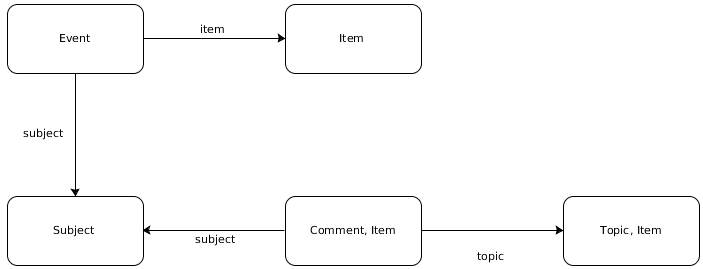
\includegraphics[width=.8\textwidth]{img/graph-model.png}
  \caption{Graph data model}
  \label{fig:graph-model}
\end{figure}

\subsubsection{Neo4j implementation}
\label{subsubsec:neo4j-implementation}

% TODO: reference
The physical data model for Neo4j is implemented using the community-supported Neo4j.rb library, which provides Ruby and Ruby on Rails bindings to the data store.

\section{Reference queries}
\label{sec:reference-queries}

% Concurrent queries pls

In order to perform an empricial analysis on the selected data stores and the proposed physical data models, we present five reference queries in this chapter.
These reference queries will reflect the method of querying that would be the most common in the physical platform implementation, and mirrors the way data is queried from a database perspective.
All reference queries will be implemented using the available language bindings, however the generated implementation-specific query will also be presented.

Since the data of the use case is aimed at a write-once, read-many character, the majority of queries will not touch the data itself, but rather only read it.
Four read-only queries are included in the following sections, and one query that will insert new data into the data store.

\subsection{Querying}
\label{subsec:querying}

\subsubsection{Query 1}
\label{subsubsec:query-1}

``
Select N most recent events, ordered reverse chronologically
''

This query, as most simple reference query presented, is an example of a query that can be used on the homepage of the platform.
% TODO: Github reference
When a user opens the web application, a reverse chronologically ordered list of events is presented, much like how the activity feed on the Github platform is structured.
This view allows for a quick overview of the activity in the platform, and since the user is not signed in yet, it is not tailored.
This also means that everyone who visits the platform without signing in will receive the same events in their Recent Activity feed.

\subsubsection*{MongoDB}

\begin{minted}{ruby}
MongoDB::Event
  .all
  .order_by(:created_at => :desc)
  .limit(count)
  .each(&:to_s)
\end{minted}

\subsubsection*{CouchDB}

% TODO

\subsubsection*{Neo4j}

\begin{minted}{ruby}
Neo4j::Event
  .all
  .order(:created_at => :desc)
  .limit(count)
  .each(&:to_s)
\end{minted}

\begin{minted}{cypher}
MATCH (result_neo4jevent:`Event`)
  RETURN result_neo4jevent
  ORDER BY result_neo4jevent.created_at DESC
  LIMIT {limit_1} | {:limit_1=>count}

MATCH (previous:`Event`)
  WHERE (ID(previous) = {ID_previous})
  OPTIONAL MATCH (previous)-[rel1:`by`]->(next:`Subject`)
  RETURN
    ID(previous),
    collect(next) | {:ID_previous=>result_neo4jevent.id}

MATCH (previous:`Event`)
  WHERE (ID(previous) = {ID_previous})
  OPTIONAL MATCH (previous)-[rel1:`on`]->(next:`Item`)
  RETURN
    ID(previous),
    collect(next) | {:ID_previous=>result_neo4jevent.id}
\end{minted}

The Neo4j ORM call get converted into three distinct queries: one to get the \texttt{Event} node and two queries to get the related nodes \texttt{Subject} and \texttt{Item}.

\subsubsection{Query 2}
\label{subsubsec:query-2}

``
Select N most recent events, where the event is related to a topic in a list of given topics, ordered reverse chronologically
''

As mentioned in chapter \TODO{??}, a user also has to ability to subscribe to topics.
Once the user logs in to the platform, the Recent Activity feed can be presented in a more attractive way.
The events in the feed will then consist of only events related to topics the user has subscribed to (which also includes the topics where the user is author or contributor).

\subsubsection*{MongoDB}

\begin{minted}{ruby}
# List of subscribed topic identifiers
topic_ids = [...]

MongoDB::Event
  .in('item._id' => topic_ds)
  .order_by(:created_at => :desc)
  .limit(count)
  .each(&:to_s)
\end{minted}

\subsubsection*{CouchDB}

% TODO

\subsubsection*{Neo4j}

\begin{minted}{ruby}
# List of subscripted topic identifiers
topic_ids = [...]

Neo4j::Topic
  .where(:id => topic_ids)
  .events
  .order_by(:created_at => :desc)
  .limit(count)
  .each(&:to_s)
\end{minted}

\begin{minted}{cypher}
MATCH (node2:`Topic`:`Item`)
  WHERE (node2.uuid IN {node2_uuid})
  MATCH (node2)<-[rel1:`on`]-(result_events:`Event`)
  RETURN result_events
  ORDER BY result_events.created_at DESC
  LIMIT {limit_1} | {:limit_1=>1, :node2_uuid=>topic_ids}

MATCH (previous:`Event`)
  WHERE (ID(previous) = {ID_previous})
  OPTIONAL MATCH (previous)-[rel1:`by`]->(next:`Subject`)
  RETURN
    ID(previous),
    collect(next) | {:ID_previous=>node2.id}

MATCH (previous:`Event`)
  WHERE (ID(previous) = {ID_previous})
  OPTIONAL MATCH (previous)-[rel1:`on`]->(next:`Item`)
  RETURN
    ID(previous),
    collect(next) | {:ID_previous=>node2.id}
\end{minted}

\subsubsection{Query 3}
\label{subsubsec:query-3}

``
Select N most recent events, where the event is related to a given topic, ordered reverse chronologically
''

Every topic also has an overview page, which mainly contains metadata such as description, author, contributors and other information not directly related to the course content.
Next to the metadata, a custom Recent Activity feed is also included on the page.
This feed only contains events related to the topic the user is currently viewing, and effectively presents a timeline of changes and discussions.

\subsubsection*{MongoDB}

\begin{minted}{ruby}
# Topic identifier
topic_id = ...

MongoDB::Event
  .where('item._id' => topic_id)
  .order_by(:created_at => :desc)
  .limit(count)
  .each(&:to_s)
\end{minted}

\subsubsection*{CouchDB}

% TODO

\subsubsection*{Neo4j}

\begin{minted}{ruby}
# Topic identifier
topic_id = ...

Neo4j::Topic
  .find(topic_id)
  .events
  .order(:created_at => :desc)
  .limit(count)
  .each(&:to_s)
\end{minted}

\begin{minted}{cypher}
MATCH (neo4j_topic)
  WHERE (ID(neo4j_topic) = {ID_neo4j_topic})
  MATCH (neo4j_topic)<-[rel1:`on`]-(result_events:`Event`)
  RETURN result_events
  ORDER BY result_events.created_at DESC
  LIMIT {limit_1} | {:limit_1=>1, :ID_neo4j_topic=>topic_id}

MATCH (previous:`Event`)
  WHERE (ID(previous) = {ID_previous})
  OPTIONAL MATCH (previous)-[rel1:`by`]->(next:`Subject`)
  RETURN
    ID(previous),
    collect(next) | {:ID_previous=>neo4j_topic.id}

MATCH (previous:`Event`)
  WHERE (ID(previous) = {ID_previous})
  OPTIONAL MATCH (previous)-[rel1:`on`]->(next:`Item`)
  RETURN
    ID(previous),
    collect(next) | {:ID_previous=>neo4j_topic.id}
\end{minted}

\subsubsection{Query 4}
\label{subsubsec:query-4}

``
Select N most recent events, where the event is related to a given user, ordered reverse chronologically
''

Similarly to topics, a user's profile page also includes a timeline of \TODO{his/her} activities: additions, deletions, comments and annotations that were recently made by that user.

\subsubsection*{MongoDB}

\begin{minted}{ruby}
# Subject identifier
subject_id = ...

MongoDB::Event
  .where('subject._id' => subject_id)
  .order_by(:created_at => :desc)
  .limit(count)
  .each(&:to_s)
\end{minted}

\subsubsection*{CouchDB}

% TODO

\subsubsection*{Neo4j}

\begin{minted}{ruby}
# Subject identifier
subject_id = ...

Neo4j::Subject
  .find(subject_id)
  .events
  .order(:created_at => :desc)
  .limit(count)
  .each(&:to_s)
\end{minted}

\begin{minted}{cypher}
MATCH (n:`Subject`)
  WHERE (n.uuid = {n_uuid})
  RETURN n
  ORDER BY n.uuid
  LIMIT {limit_1} | {:n_uuid=>subject_id, :limit_1=>1}

MATCH (neo4j_subject)
  WHERE (ID(neo4j_subject) = {ID_neo4j_subject})
  MATCH (neo4j_subject)<-[rel1:`by`]-(result_events:`Event`)
  RETURN result_events
  ORDER BY result_events.created_at DESC
  LIMIT {limit_1} | {:limit_1=>1, :ID_neo4j_subject=>subject_id}

MATCH (previous:`Event`)
  WHERE (ID(previous) = {ID_previous})
  OPTIONAL MATCH (previous)-[rel1:`by`]->(next:`Subject`)
  RETURN
    ID(previous),
    collect(next) | {:ID_previous=>result_events.id}

MATCH (previous:`Event`)
  WHERE (ID(previous) = {ID_previous})
  OPTIONAL MATCH (previous)-[rel1:`on`]->(next:`Item`)
  RETURN
    ID(previous),
    collect(next) | {:ID_previous=>result_events.id}
\end{minted}

\subsection{Insertion}
\label{subsec:insertion}

\subsubsection{Query 5}
\label{subsubsec:query-5}

``
Insert N given :created or :updated events
''

Finally, since read requests will most likely outnumber write requests with several magnitudes in the studied use case, only one query where data is inserted is presented.
The query creates a single event in the data store.

\subsubsection*{MongoDB}

\begin{minted}{ruby}
# Subject identifier
subject_id = ...

# Item identifier
item_id = ...

MongoDB::Event.create! :subject => subject_id,
                       :item => item_id,
                       :predicate => :updated
\end{minted}

\subsubsection*{CouchDB}

% TODO

\subsubsection*{Neo4j}

\begin{minted}{ruby}
# Subject identifier
subject_id = ...

# Item identifier
item_id = ...

Neo4j::Event .create! :subject => subject_id,
                      :item => topic_id,
                      :predicate => :updated
\end{minted}

\begin{minted}{cypher}
MATCH (n:`Subject`)
  WHERE (n.uuid = {n_uuid})
  RETURN n
  ORDER BY n.uuid
  LIMIT {limit_1} | {:n_uuid=>subject_id, :limit_1=>1}

MATCH (n:`Item`)
  WHERE (n.uuid = {n_uuid})
  RETURN n
  ORDER BY n.uuid
  LIMIT {limit_1} | {:n_uuid=>item_id, :limit_1=>1}

CREATE (n:`Event`)
  SET n = {props}
  RETURN n | {:props=>{:uuid=>event_id, :created_at=>1526737892, :predicate=>1}}

MATCH (n:`Subject`)
  WHERE (n.uuid = {n_uuid})
  RETURN n
  LIMIT {limit_1} | {:n_uuid=>subject_id, :limit_1=>1}

MATCH
    (from_node),
    (to_node)
  WHERE
    (ID(from_node) = {ID_from_node}) AND
    (ID(to_node) = {ID_to_node})
  CREATE (from_node)-[rel:`by` {rel_create_props}]->(to_node)
    | {:ID_from_node=>event_id, :ID_to_node=>subject_id, :rel_create_props=>{}}

MATCH (n:`Item`)
  WHERE (n.uuid = {n_uuid})
  RETURN n
  LIMIT {limit_1} | {:n_uuid=>item_id, :limit_1=>1}

MATCH
    (from_node),
    (to_node)
  WHERE
    (ID(from_node) = {ID_from_node}) AND
    (ID(to_node) = {ID_to_node})
  CREATE (from_node)-[rel:`on` {rel_create_props}]->(to_node)
    | {:ID_from_node=>event_id, :ID_to_node=>item_id, :rel_create_props=>{}}

\end{minted}

\section{Conclusion}
\label{sec:data-model-conclusion}

In this chapter we presented an introduction to the domain, and provided some examples of events in the Recent Activity feed.
Futhermore, we analyzed this domain description, and derived a logical data model for both document- and graph-oriented data stores.
Next, we proposed an implementation of this logical data model for two document-oriented, and one graph-oriented data store in the Ruby language bindings available for the respective database management systems.
Finally, we presented five reference queries for the three data stores, and included both a language binding-specific DSL and a physical query implementation for each.

% TODO: Conclusion about ORMs
